\documentclass{beamer}
\usetheme{Antibes}
\usecolortheme{dove}

\usepackage{beamerthemesplit}
\usepackage{graphics}
\usepackage{graphicx}
\usepackage{hyperref}

\title{Parallelizing a Traffic Simulation}
\author{Venelin Valkov}
\institute[University of Plovdiv]{Faculty of Mathematics and Informatics\\University of Plovdiv}
\date{1 March, 2012}
\subject{OpenCL Simulation}

\begin{document}

  \frame
  {
    \titlepage
  }

  \section*{Contents}

  \frame
  {
    \frametitle{Contents}

    \tableofcontents
  }

  \section{Why a simulation?}

  \frame
  {
    \frametitle{Why a simulation?}

    Real world is always much more fun than the imaginary one. However, sometimes it is better to test in the second one
  }
  
  \section{Traffic all around us, literally!}
  \frame
  {
  	\frametitle{Traffic all around us, literally!}
  	\begin{itemize}
  		\item Public transportation user? It is sooo slow!
  		\item You have a car? Well I don't!
  		\item Why not take a walk? Wonderful idea, not everybody can afford that though
	\end{itemize}
}
  \section{Parallelism is easy, right?}
  \frame
  {
  	\frametitle{Parallelism is easy, right?}
  	What we need?
  	\begin{itemize}
  		\item Fast computers
  		\item Cool new technology to play with
  		\item Free time
	\end{itemize}  	
  }  
  
  \frame
  {
    \frametitle{But what if you have only the technology?}
	\begin{figure}
      \scalebox{0.50}
      {
        
\includegraphics{opencl.png}
      }
            \scalebox{0.30}
      {
        
\includegraphics{cuda.jpg}
      }
    \end{figure}
  }
  
  \frame
  {
	\frametitle{Welcome to OpenCL}
    \begin{itemize}
    \item<1-> Open specification
    \item<2-> Proposed by Apple
    \item<3-> Maintained by Khronos Group
    \item<4-> Heterogeneous Computing
    \item<5-> Write once, run everywhere (yeah... almost)      
    \end{itemize}  
  }

  \section{Parallelism Overview}

  \frame
  {
  	\begin{figure}
        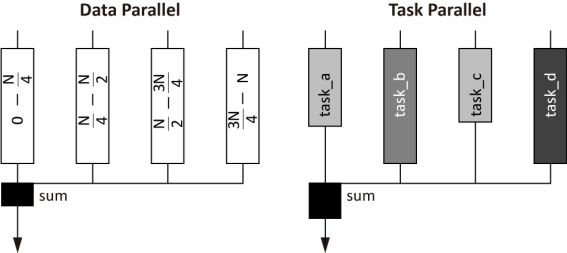
\includegraphics{parallelism-types.jpg}
    \end{figure}
  }

  \section{What's next?}

  \frame
  {
    \frametitle{What's next?}

    \begin{itemize}
    \item<1-> Come up with a mathematical model for the simulation ( or better yet - steal one )
    \item<2-> Writing some code is never bad idea
    \item<3-> Design a fancy UI for the jury
    \end{itemize}
  }
  
  \frame
  {
	\frametitle{Thanks!}
	\begin{center}
		\Large \emph{The End}
	\end{center}
  }
  
  \frame
  {
	\frametitle{Resources}  
	\begin{itemize}
	  	\item \href{http://www.khronos.org/opencl/} Khronos Group official OpenCL page
  		\item \href{http://www.fixstars.com/en/opencl/book/OpenCLProgrammingBook/dtp_462724_USER_CONTENT_0_html_m3285f80d.jpg} OpenCL diagram
  		\item \href{http://www.khronos.org/assets/uploads/developers/library/overview/opencl-overview.pdf} OpenCL Overview
	\end{itemize}	  
  }

\end{document}
